\documentclass[DIV=15,
fleqn
numbers=noenddot,
headsepline,
captions=tableabove,twoside, openright]{scrreprt}
\usepackage{pgf,tikz}
\usepackage[utf8]{inputenc}
\usepackage[T1]{fontenc}
\usepackage[english]{babel}
\usepackage[intlimits,slantedGreeks]{kpfonts}
\usepackage[expansion=false]{microtype}
\usepackage{bm}
\usepackage[]{graphicx}
\usepackage{psfrag}\usepackage{amsmath}
\usepackage{amsfonts}
\usepackage{amssymb}
\usepackage{graphics}
\usepackage{color}
\usepackage{colortbl, hhline}
\usepackage{subfigure}
\usepackage{float}
\usepackage{url}
\usepackage{upgreek}
\usepackage{multicol,caption}
\usepackage[titletoc]{appendix}
\usepackage{mathtools}
\usepackage{amsmath}
\usepackage{calc}
\usepackage{epstopdf}
\usepackage{units}
\usepackage{tabularx}
\usepackage{booktabs}
\usepackage{longtable}
\usepackage{listings}
\usepackage[automark]{scrpage2}
\usepackage{babelbib}
\usepackage{tikz}
%-----------------NEW PACKAGES from October2017--------%
\usepackage[]{datetime2}
\usepackage{enumitem}
\setlist[description]{leftmargin=2cm,labelindent=2cm}
\usepackage{acro}
\DeclareAcronym{mimo}{
	short = MIMO,
	long = Multiple-Input Multiple-Output}
\usepackage{cleveref}
\DeclareAcronym{fmcw}{
	short = FMCW,
	long = Frequency-Modulated Continuous-Wave}
\DeclareAcronym{if}{
	short = IF , long =
	intermediate frequency }
\DeclareAcronym{fft}{
	short = FFT , long = Fast Fourier Transform }
\DeclareAcronym{mtt}{
	short =MTT,
    long = Multi-Target Tracking }
\DeclareAcronym{lti}{
	short = LTI , long = Linear Time Invariant}
%ausprobieren
\setcounter{secnumdepth}{2}
\setcounter{tocdepth}{2}
%ausprobieren ende




\pagestyle{scrplain}
\clearscrheadfoot
\ihead{}
\chead{}
\ohead{}
\ifoot{}
\cfoot[\pagemark]{\pagemark}
\ofoot{}

	

\setkomafont{disposition}     {\normalfont\bfseries}
\setkomafont{descriptionlabel}{\normalfont\bfseries}
\setkomafont{pagehead}        {\normalfont}
\setkomafont{caption}         {\normalfont\small}
\setkomafont{captionlabel}    {\normalfont\small\bfseries}
\setcapindent{0em}

\setcounter{secnumdepth}{3}
\setcounter{tocdepth}{3}

\setcounter{topnumber}           {1}
\setcounter{bottomnumber}        {1}
\renewcommand{\floatpagefraction}{0.8}
\renewcommand{\topfraction}      {0.8}
\renewcommand{\bottomfraction}   {0.5}
\renewcommand{\textfraction}     {0.15}
\makeatletter
\setlength{\@fptop}{0pt}
\makeatother
%--------------------Command definitions--------------%
\newcommand*{\mj}   {\mathrm{j}}
\newcommand*{\me}   {\mathrm{e}}
\newcommand*{\Div}  {\operatorname{div}}
\newcommand*{\Rot}  {\operatorname{rot}}
\newcommand*{\Grad} {\operatorname{grad}}
\renewcommand*{\Re} {\operatorname{Re}}
\renewcommand*{\Im} {\operatorname{Im}}
\renewcommand{\Re}  {\operatorname{Re}}
\renewcommand{\Im}  {\operatorname{Im}}
\renewcommand{\vec}   [1]{\bm{#1}}
\renewcommand{\matrix}[1]{\mathbf{#1}}
\newcommand* {\snr} {\mathrm{SNR}}
\newcommand{\Iog}  {\operatorname{log}}


\addto\captionsenglish{%
	\renewcommand{\figurename}{Figure}%
}


\AtBeginDocument{\bbbbaddto{english} {btxifchangecaseoff}}
\bibliographystyle{unsrt}
\usepackage{titlesec}


\usetikzlibrary{arrows}


%------------------Date Settings------------------------%
\DTMsetdatestyle{ddmmyyyy}

\begin{document}
%---------------------COVER------------------------------%
\input{cover/cover}
%-------------------FIRST PAGES-------------------------%

\pagenumbering{Roman}
\chapter*{Sperrvermerk}

\chapter*{Declaration of Authorship}
\chapter*{}
\vspace*{8cm}
\thispagestyle{empty}
%------------------DEDICATION--------------------------------%
\input{cover/Dedication}
%--------------------Contents--------------------------------%
\tableofcontents	
%***********************************************
%INTRODUCTION
%***********************************************
\chapter{Introduction}
	\pagenumbering{arabic}
	\pagestyle{scrheadings}
	\clearscrheadfoot
	\ihead{\headmark}
	\ohead{\pagemark}
	
\chapter{Radar Fundamentals}\label{ch:basics}
\begin{figure}[h!]
	\centering
	
\begin{tikzpicture}
% Reference Grid
\draw[gray,very thin] (0,0) grid (10,4); 

\end{tikzpicture}
	\caption{Block Diagram of the whole process}
	\label{fig:intro}
\end{figure} 
\section{Radar Definitions}\label{bs:definitions}
 Range
\begin{equation}
	R = \frac{c_0\Delta t}{2}
\end{equation}
Pulse repetition interval (PRI)
\begin{equation}
	f_r = \frac{1}{T}
\end{equation}
Unambiguous range  $R_u$
\begin{figure}
	\centering
	
\begin{tikzpicture}
% Reference Grid
\draw[gray,very thin] (0,0) grid (10,4); 

\end{tikzpicture}
	\caption{Illustrating the unambiguous range}
\end{figure} 
 \section{MIMO Array}\label{bs:MIMO}
 For the estimation of the azimuth and elevation of a target's position, the phase array radar has been a popular choice during the past decades. This technique employs a series of antennas to transmit and receive the electromagnetic waveform before mentioned. Here, the phase of each element in the group of transmitted is adjusted for the radar to be able to suppress the response from specific directions and thus, "scan" a specific direction. The angular resolution of this method, however, strongly depends on the number of elements in the antenna array. An attractive alternative to the simple phase array is its combination with the \ac{mimo} concept \cite{fishler_mimo_2004}. 

As the name implies, a \ac{mimo} radar consists of multiple transmit (TX) antennas and receive (RX) antennas. $M_t$ transmit and $M_r$ receive elements are assumed. The difference from the phase array radar is that the signals transmitted by each of the TX elements are diversified, leading to $M_t\times M_r$ propagation channels. This, with only $M_t + M_r$ antenna elements. With this concept, a higher performance with a substantially lower cost can be achieved, which is why the \ac{mimo} array has been chosen for the purpose of this thesis. 

Several methods to the define the diversity of the TX channels have been proposed, these include frequency division multiplexing, spatial coding, orthogonal waveforms and time division multiplexing. The latter has been chosen and implemented as presented in \cite{huang_fmcw_2011}. As the name indicates and as presented in \cref{fig:tdm}, the concept time division multiplexing consists in switching the transmit antenna at each consecutive pulse. Hereby, one is able to differentiate at the receiver from which TX element is the signal coming simply by looking at the time of reception, which is important for the estimation of the azimuth profile (\cref{bs:azimuth}).


\begin{figure}[h!]
	\centering
	
\begin{tikzpicture}
% Reference Grid
\draw[gray,very thin] (0,0) grid (10,4); 

\end{tikzpicture}
	\caption{Time division multiplexing for \Ac{mimo}-radar.}
	\label{fig:tdm}
\end{figure} 


A further design concern is the array manifold. Different array forms can be found in literature, where the most common are the uniform linear array (ULA) and the uniform circular array (UCA) \cite{zhang_blind_2009}, which are depicted in \cref{fig:ula,fig:uca}. As the name indicates, this manifolds consists of equidistant antenna elements in either linear or circular form. The MIMO-radar chosen here consists in 2 TX and 4 RX array resulting in 8 virtual channels.

\begin{figure}[h!]
	\centering
	\begin{minipage}{.5\textwidth}
		\centering
		
\begin{tikzpicture}
% Reference Grid
\draw[gray,very thin] (0,0) grid (7,5); 

\end{tikzpicture}
		\captionof{figure}{Uniform Linear Array (ULA).}
		\label{fig:ula}
	\end{minipage}%
	\begin{minipage}{.5\textwidth}
		\centering
		
\begin{tikzpicture}
% Reference Grid
\draw[gray,very thin] (0,0) grid (7,5); 

\end{tikzpicture}
		\captionof{figure}{Uniform Circular Array (UCA).}
		\label{fig:uca}
	\end{minipage}
\end{figure}

If the far-field condition is satisfied, the \Ac{mimo}-configuration can be modeled as an ULA of  $M_t\times M_r$ virtual antennas. Given the position of the TX-elements $x_i^{Tx}$ and RX-elements $x_j^{Rx}$ the virtual ULA is modeled by antenna elements at 

\begin{equation}
\vec{x_{ij}} = (\vec{x}_i^{Tx}+\vec{x}_j^{Rx})/2\\,
\end{equation}
for $i = 1,...,M_t$ and $j = 1,...,M_r$. Presented in \cref{fig:mimo_array} is a \Ac{mimo}-setup with its corresponding virtual elements. Note that for this work the TX and RX elements are aligned in the vertical axis. This has been ignored here for better illustration. 

\begin{figure}[h]
	\centering
	For the estimation of the azimuth and elevation of a target's position, the phase array radar has been a popular choice during the past decades. This technique employs a series of antennas to transmit and receive the electromagnetic waveform before mentioned. Here, the phase of each element in the group of transmitted is adjusted for the radar to be able to suppress the response from specific directions and thus, "scan" a specific direction. The angular resolution of this method, however, strongly depends on the number of elements in the antenna array. An attractive alternative to the simple phase array is its combination with the \ac{mimo} concept \cite{fishler_mimo_2004}. 

As the name implies, a \ac{mimo} radar consists of multiple transmit (TX) antennas and receive (RX) antennas. $M_t$ transmit and $M_r$ receive elements are assumed. The difference from the phase array radar is that the signals transmitted by each of the TX elements are diversified, leading to $M_t\times M_r$ propagation channels. This, with only $M_t + M_r$ antenna elements. With this concept, a higher performance with a substantially lower cost can be achieved, which is why the \ac{mimo} array has been chosen for the purpose of this thesis. 

Several methods to the define the diversity of the TX channels have been proposed, these include frequency division multiplexing, spatial coding, orthogonal waveforms and time division multiplexing. The latter has been chosen and implemented as presented in \cite{huang_fmcw_2011}. As the name indicates and as presented in \cref{fig:tdm}, the concept time division multiplexing consists in switching the transmit antenna at each consecutive pulse. Hereby, one is able to differentiate at the receiver from which TX element is the signal coming simply by looking at the time of reception, which is important for the estimation of the azimuth profile (\cref{bs:azimuth}).


\begin{figure}[h!]
	\centering
	
\begin{tikzpicture}
% Reference Grid
\draw[gray,very thin] (0,0) grid (10,4); 

\end{tikzpicture}
	\caption{Time division multiplexing for \Ac{mimo}-radar.}
	\label{fig:tdm}
\end{figure} 


A further design concern is the array manifold. Different array forms can be found in literature, where the most common are the uniform linear array (ULA) and the uniform circular array (UCA) \cite{zhang_blind_2009}, which are depicted in \cref{fig:ula,fig:uca}. As the name indicates, this manifolds consists of equidistant antenna elements in either linear or circular form. The MIMO-radar chosen here consists in 2 TX and 4 RX array resulting in 8 virtual channels.

\begin{figure}[h!]
	\centering
	\begin{minipage}{.5\textwidth}
		\centering
		
\begin{tikzpicture}
% Reference Grid
\draw[gray,very thin] (0,0) grid (7,5); 

\end{tikzpicture}
		\captionof{figure}{Uniform Linear Array (ULA).}
		\label{fig:ula}
	\end{minipage}%
	\begin{minipage}{.5\textwidth}
		\centering
		
\begin{tikzpicture}
% Reference Grid
\draw[gray,very thin] (0,0) grid (7,5); 

\end{tikzpicture}
		\captionof{figure}{Uniform Circular Array (UCA).}
		\label{fig:uca}
	\end{minipage}
\end{figure}

If the far-field condition is satisfied, the \Ac{mimo}-configuration can be modeled as an ULA of  $M_t\times M_r$ virtual antennas. Given the position of the TX-elements $x_i^{Tx}$ and RX-elements $x_j^{Rx}$ the virtual ULA is modeled by antenna elements at 

\begin{equation}
\vec{x_{ij}} = (\vec{x}_i^{Tx}+\vec{x}_j^{Rx})/2\\,
\end{equation}
for $i = 1,...,M_t$ and $j = 1,...,M_r$. Presented in \cref{fig:mimo_array} is a \Ac{mimo}-setup with its corresponding virtual elements. Note that for this work the TX and RX elements are aligned in the vertical axis. This has been ignored here for better illustration. 

\begin{figure}[h]
	\centering
	For the estimation of the azimuth and elevation of a target's position, the phase array radar has been a popular choice during the past decades. This technique employs a series of antennas to transmit and receive the electromagnetic waveform before mentioned. Here, the phase of each element in the group of transmitted is adjusted for the radar to be able to suppress the response from specific directions and thus, "scan" a specific direction. The angular resolution of this method, however, strongly depends on the number of elements in the antenna array. An attractive alternative to the simple phase array is its combination with the \ac{mimo} concept \cite{fishler_mimo_2004}. 

As the name implies, a \ac{mimo} radar consists of multiple transmit (TX) antennas and receive (RX) antennas. $M_t$ transmit and $M_r$ receive elements are assumed. The difference from the phase array radar is that the signals transmitted by each of the TX elements are diversified, leading to $M_t\times M_r$ propagation channels. This, with only $M_t + M_r$ antenna elements. With this concept, a higher performance with a substantially lower cost can be achieved, which is why the \ac{mimo} array has been chosen for the purpose of this thesis. 

Several methods to the define the diversity of the TX channels have been proposed, these include frequency division multiplexing, spatial coding, orthogonal waveforms and time division multiplexing. The latter has been chosen and implemented as presented in \cite{huang_fmcw_2011}. As the name indicates and as presented in \cref{fig:tdm}, the concept time division multiplexing consists in switching the transmit antenna at each consecutive pulse. Hereby, one is able to differentiate at the receiver from which TX element is the signal coming simply by looking at the time of reception, which is important for the estimation of the azimuth profile (\cref{bs:azimuth}).


\begin{figure}[h!]
	\centering
	\input{fundamentals_figs/blank.tex}
	\caption{Time division multiplexing for \Ac{mimo}-radar.}
	\label{fig:tdm}
\end{figure} 


A further design concern is the array manifold. Different array forms can be found in literature, where the most common are the uniform linear array (ULA) and the uniform circular array (UCA) \cite{zhang_blind_2009}, which are depicted in \cref{fig:ula,fig:uca}. As the name indicates, this manifolds consists of equidistant antenna elements in either linear or circular form. The MIMO-radar chosen here consists in 2 TX and 4 RX array resulting in 8 virtual channels.

\begin{figure}[h!]
	\centering
	\begin{minipage}{.5\textwidth}
		\centering
		\input{fundamentals_figs/blank2.tex}
		\captionof{figure}{Uniform Linear Array (ULA).}
		\label{fig:ula}
	\end{minipage}%
	\begin{minipage}{.5\textwidth}
		\centering
		\input{fundamentals_figs/blank2.tex}
		\captionof{figure}{Uniform Circular Array (UCA).}
		\label{fig:uca}
	\end{minipage}
\end{figure}

If the far-field condition is satisfied, the \Ac{mimo}-configuration can be modeled as an ULA of  $M_t\times M_r$ virtual antennas. Given the position of the TX-elements $x_i^{Tx}$ and RX-elements $x_j^{Rx}$ the virtual ULA is modeled by antenna elements at 

\begin{equation}
\vec{x_{ij}} = (\vec{x}_i^{Tx}+\vec{x}_j^{Rx})/2\\,
\end{equation}
for $i = 1,...,M_t$ and $j = 1,...,M_r$. Presented in \cref{fig:mimo_array} is a \Ac{mimo}-setup with its corresponding virtual elements. Note that for this work the TX and RX elements are aligned in the vertical axis. This has been ignored here for better illustration. 

\begin{figure}[h]
	\centering
	\input{fundamentals_figs/mimo.tex}
	\caption{\ac{mimo}-array}
		\label{fig:mimo_array}
\end{figure} 
 
 Under the described conditions the signal propagation path from a given TX element to a scatterer at point $\vec{p}$, plus the reflection path back to an RX element can be approximated as
 \begin{equation}
 	P_{ij}(p) = |\vec{p}-\vec{x}_i^{Tx}| + |\vec{p}-\vec{x}_j^{Rx}| \approx 2|\vec{p}-\vec{x}_{ij}| \\.
 \end{equation}
	\caption{\ac{mimo}-array}
		\label{fig:mimo_array}
\end{figure} 
 
 Under the described conditions the signal propagation path from a given TX element to a scatterer at point $\vec{p}$, plus the reflection path back to an RX element can be approximated as
 \begin{equation}
 	P_{ij}(p) = |\vec{p}-\vec{x}_i^{Tx}| + |\vec{p}-\vec{x}_j^{Rx}| \approx 2|\vec{p}-\vec{x}_{ij}| \\.
 \end{equation}
	\caption{\ac{mimo}-array}
		\label{fig:mimo_array}
\end{figure} 
 
 Under the described conditions the signal propagation path from a given TX element to a scatterer at point $\vec{p}$, plus the reflection path back to an RX element can be approximated as
 \begin{equation}
 	P_{ij}(p) = |\vec{p}-\vec{x}_i^{Tx}| + |\vec{p}-\vec{x}_j^{Rx}| \approx 2|\vec{p}-\vec{x}_{ij}| \\.
 \end{equation}
\section{Signal Model}\label{bs:signal}
For the following analyses a \Ac{fmcw} Radar is taken into consideration. The TX array elements transmit a \Ac{fmcw} chirp signal, that can be modeled in as
\begin{equation}
	s_T(t) = \exp[\mj(2\pi f_ct+\pi kt^2)]\\,
\end{equation}
for $-T_c/2 \leq t \leq T_c/2$, where $T_c$ is the chirp duration, $f_c$ the carrier frequency and the chirp rate $k$ is defined by
\begin{equation}
	k = \pm B/T_c\\.
\end{equation}
Under far-field condition, the return delay between a virtual element at $x_{ij}$ and a scatterer is given by
\begin{equation}
	\Delta t_{ij} = \frac{2R}{c_0} + \frac{2x_{ij}\sin\theta}{c_0}\\,
\end{equation}
where $R$ and $\theta$ describe the location of the scatterer, $R$ being the rang and $\theta$ the angle with respect to boresight. The received signal 
\begin{equation}
	s_R^{ij}(t) = As_t(t-\Delta t_{ij})
\end{equation}
After the signal is received, it is down-converted by multiplying it with a replica of the transmitted signal. After low-pass filtering, the processed signal can be modeled as 
\begin{equation}
	u_{ij}(t) = s_R^{ij}s_T(t) = A\exp[\mj(2\pi k \Delta t_{ij}t-\pi k\Delta  t_{ij}^2 + 2\pi f_c \Delta t_{ij})]
\end{equation}
The sampled form of the \ac{if} signal given $N$ samples can be expressed as
\begin{equation}
	u_{ij}[n] = A\exp[\mj(\phi+2\pi\Psi_R n)]\\,
\end{equation}
with $\Psi_R = k\Delta t_{ij}\frac{T_c}{N} $,the normalized frequency containing the range information and $\phi = -\pi k\Delta  t_{ij}^2 + 2\pi f_c \Delta t_{ij} $ contains the phase information. This expression can be generalized to \ac{mimo} radar, with $M$ targets either static or dynamic, for the $k$-th observation interval by
\begin{equation}\label{eq:signal}
	u_{k}[n,n_C,n_A] = \sum_{m=0}^{M}A_m\exp[\mj2\pi(\phi_m+\Psi_{R,m}n+\Psi_{D,m}n_C+\Psi_{\theta,m}n_A)] + w[n,n_C,n_A]
\end{equation}
where $\Psi_D = \frac{2T_cf_0}{c_0}v_R$ and $\Psi_\theta =\sin(\theta)/2 $ are the normalized frequencies containing the information about range-rate and azimuth. Moreover, $w[n,n_C,n_A]$ is the present additive white Gaussian measurement noise. The parameters $n$, $n_C$ and $n_A$ represent which, sample chirp and antenna is being taken into account. Please note that $\phi_m$ does not correspond to $\phi$.

The information collected from \cref{eq:signal} is usually arrange into a three-dimensional data cube as presented in \cref{fig:datacube}. Here the dimensions correspond to sample number, transmit-receive channel and chirp number. 

\begin{figure}[h]
	\centering
	
\begin{tikzpicture}
% Reference Grid
\draw[gray,very thin] (0,0) grid (10,4); 

\end{tikzpicture}
	\caption{Data Cube}
	\label{fig:datacube}
\end{figure} 

In order to estimate the spectrum of the received signal and so to determine the unknown parameters $R$, $v_R$ and $\theta$ for a given target, usually a three-dimensional \ac{fft} is applied to de \Ac{if} signal
\begin{multline}
\hat{P}_k(\Psi_R,\Psi_D\Psi_\theta) = \sum_{n}\sum_{n_C}\sum_{n_A} a_R[n] a_D[n_C] a_\theta[n_A]u_k[n,n_A,n_C]\\
\times\exp(-\mj2\pi\Psi_Rn)\exp(-\mj2\pi\Psi_Dn_C)\exp(-\mj2\pi\Psi_\theta n_A) \rlap{,}
\end{multline}
however, this usually results in a bad estimation for the azimuth range. Specifics of the signal processing will be described in the following sections. 

\section{Ranging}\label{bs:ranging}
\section{Doppler Ranging}\label{bs:dopplerRanging}
\section{Azimuth Estimation}
\section{Detection Theory}\label{bs:detection}
\chapter{Clustering}
\chapter{Multi-Target Tracking}
After a correct detection and clustering of targets, the detections have to be assigned to tracks which are to be updated over time. In this case, it is done to create a history of each of the target's range, azimuth angle and Doppler velocity. In a further step, the Micro-Doppler signature can be extracted from each of the tracks and be used as an input for the classifiers. More over, by keeping track of the measurements corresponding to each track, one can produce an estimate of future positions of the target, which result into a more accurate measurement of the targets position. This process is called \ac{mtt}.

Each track of a \ac{mtt}-algorithm contains a Kalman Filter (\cref{mtt:kalman}) which is a commonly used filter to predict future states and to calculate variables that cannot be measured directly. At each step, gating (\cref{mtt:gating}) is applied to each of the new detections to reduce the scope of detections that can be assigned to a given track at each time step $k$. After gating, the detections calculated in a given step are assigned to each of the tracks. For this, the assignment problem has to be solved (\cref{mtt:assign}). After the assignment has been done, the state of each of the tracks is updated according to pre-established rules (\cref{mtt:management}). The whole process used for the \ac{mtt} is illustrated in \cref{fig:mtt}.
\begin{figure}[h]
	\centering
	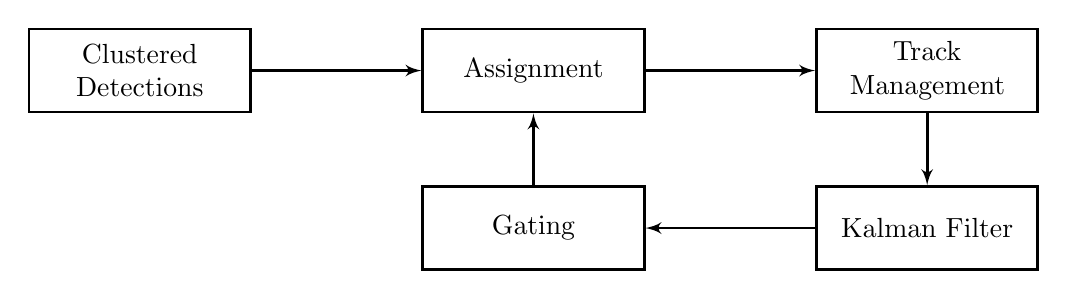
\begin{tikzpicture}[auto,>=latex']
%\draw[gray,very thin] (0,0) grid (15,4); s
   \tikzstyle{block} = [draw, shape=rectangle, minimum height=3em, minimum width=8em, node distance=2cm, line width=1pt]
\tikzstyle{sum} = [draw, shape=circle, node distance=1.5cm, line width=1pt, minimum width=1.25em]
\tikzstyle{branch}=[fill,shape=circle,minimum size=4pt,inner sep=0pt]
%Creating Blocks and Connection Nodes
\node at (3,3) [text width=2 cm,block,align = center] (input) {Clustered  Detections };
\node at (8,3) [block] (h1) {Assignment}; 
\node at (13,3)[text width=2 cm,block,align = center] (h2) {Track \\ Management}; 
\node at (13,1) [block] (h3) {Kalman Filter}; 
\node at (8,1) [block] (h4) {Gating}; 
\begin{scope}[line width = 1pt]
\draw[->] (input) -- (h1);
\draw[->] (h1)--(h2);
\draw[->] (h2) -- (h3); 
\draw[->] (h3)--(h4); 
\draw[->] (h4)--(h1); 

\end{scope}

\end{tikzpicture}
	\caption{MTT-process}
	\label{fig:mtt}
\end{figure} 
Given that usually a constant-velocity model is assumed, a special model needs to be implemented to consider the cases where the target has an (unknown) acceleration. This is issue is handled in \cref{mtt:maneuver}.
\section{State Variable Representation of an LTI System}\label{mtt:state}
A \ac{lti} system can be described by by three variables, input, output and the state variable. In the case of radar, the state can be design to contain several attributes of single targets measured by the radar such as range, range-rate and azimuth angle. Since we desire to determines a target's position and velocity in Cartesian coordinates, the state vector 
\begin{equation}
	\vec{x} = \begin{bmatrix}
	x \\ y \\ v_x \\ v_y
	\end{bmatrix}\\,
\end{equation}
has been chosen. The continuous-time linear system can then be written as
\begin{equation}
	\dot{\vec{x}}(t) = \matrix{A}(t)\vec{x}(t)+ \matrix{B}(t)\vec{u}(t) + \tilde{\vec{v}}(t)\\,
\end{equation}
where $t$ represents time and 
\begin{description}[align=left,labelwidth=1cm]
	\item[$\vec{x}$] is the state vector of dimension $n_x$ and $\dot{\vec{x}}$ its time derivative.
	\item[$\vec{u}$] is the input(or control) vector of dimension $n_u$
	\item[$\tilde{\vec{v}}$] is the process noise
	\item[$\matrix{A}$,$\matrix{B}$] are known matrices of dimensions $n_x\times n_x$ and $n_x\times n_u$
\end{description}
\section{The Kalman Filter}\label{mtt:kalman}
\section{Gating Techniques}\label{mtt:gating}
\section{The Assignment Problem}\label{mtt:assign}
\subsection{NN-approach}\label{mtt:nn}
\subsection{PDA-approach}\label{mtt:pda}
\subsection{JPDA-approach}\label{mtt:jpda}
\section{Track Life Stages}\label{mtt:management}
\section{Maneuver Detection and Adaptive Filtering}\label{mtt:maneuver}
\chapter{Micro-Doppler Signatures}
\chapter{Classification}
\chapter{Results}
\chapter{Summary and Outlook}
\begin{appendices}
\chapter{Symbols and Constants}
\section*{General}
\begin{longtable}{ p{.20\textwidth}  p{.80\textwidth} } 
% Lateinische Buchstaben
$ \oint $ & Integration over a closed curve \\
\addlinespace[15pt]
\end{longtable}
\section*{Latin alphabet}	
\begin{longtable}{ p{.20\textwidth}  p{.80\textwidth} } 
% Lateinische Buchstaben
$R$ & Range \\
$R_u$ & Unambiguous Range \\
\addlinespace[15pt]
\end{longtable}
\section*{Greek alphabet}	
\begin{longtable}{ p{.20\textwidth}  p{.80\textwidth} } 

%Griechische Buchstaben
$ \Delta T $ & Delay\\
\addlinespace[15pt]
\end{longtable}
\section*{Constants}	
\begin{longtable}{ p{.10\textwidth}  p{.075\textwidth}  p{.80\textwidth}} 
% Lateinische Buchstaben
$ c_0 $ & $=$ & \unit[299729458]{m/s} \\
\addlinespace[15pt]
\end{longtable}
\chapter{Mathematical Formulas}


\end{appendices}
\newpage

\bibliography{misreferencias}


\newpage
\end{document}
